\documentclass{article} % For LaTeX2e
\usepackage[final]{colm2025_conference}
\usepackage{graphicx}
\usepackage{amsmath}
\usepackage{microtype}
\usepackage{hyperref}
\usepackage{url}
\usepackage{booktabs}
\usepackage{lineno}
\usepackage{amsmath}
\usepackage{algpseudocode}
\usepackage{algorithm}
\usepackage{graphicx} % Required for inserting images
\usepackage{subcaption} % For subfigure arrangement
\usepackage{caption}

\definecolor{darkblue}{rgb}{0, 0, 0.5}
\hypersetup{colorlinks=true, citecolor=darkblue, linkcolor=darkblue, urlcolor=darkblue}

\usepackage{etoolbox}
\makeatletter
\patchcmd{\@maketitle}
  {Published as a conference paper at COLM 2025}
  {}
  {}
  {}
\makeatother
\title{Week 5 Report}

% Authors must not appear in the submitted version. They should be hidden
% as long as the \colmfinalcopy macro remains commented out below.
% Non-anonymous submissions will be rejected without review.

\author{Mu Junrong}

% The \author macro works with any number of authors. There are two commands
% used to separate the names and addresses of multiple authors: \And and \AND.
%
% Using \And between authors leaves it to \LaTeX{} to determine where to break
% the lines. Using \AND forces a linebreak at that point. So, if \LaTeX{}
% puts 3 of 4 authors names on the first line, and the last on the second
% line, try using \AND instead of \And before the third author name.

\newcommand{\fix}{\marginpar{FIX}}
\newcommand{\new}{\marginpar{NEW}}

\begin{document}

\ifcolmsubmission
\linenumbers
\fi

\maketitle

\begin{abstract}
This report provides a brief summary of the key contributions of the paper "Training language models to follow instructions with human feedback” by Ouyang et al. (OpenAI)(\cite{ouyang2022instructgpt}), and discusses the training model of InstructGPT which implements Reinforcement Learning from Human Feedback (RLHF). The paper also discusses the relevant work done, as well as some potential research directions.
\end{abstract}

\section{Summary of the paper}
The paper "Training language models to follow instructions with human feedback” (
\cite{ouyang2022instructgpt}) points out and addresses a major limitation of large language models (LLMs). Simply increasing the model size does not necessarily improve the model's performance (i.e., it behaves helpfully, truthfully, and safely). To better align models with human intent, the paper proposes fine-tuning using human feedback, which is the basis for the model InstructGPT.

\subsection{Key findings}
The paper has several key contributions to the field of Large Language Models (LLMs). It proves that pretraining LLMs on next-token prediction does not naturally result in models that follow instructions or behave safely. Thus, models often produce untruthful, biased, or toxic outputs. To improve on this, the paper proposed the solution of Reinforcement Learning from Human Feedback (RLHF). The paper uses a three-step process to align GPT-3 with human intent: Supervised Fine-Tuning (SFT), Reward Modeling (RM) and Reinforcement Learning (PPO). The model that implements this fine-tuning using RLHF is InstructGPT. Surprisingly, the 1.3B parameter InstructGPT was preferred by human evaluators over the 175B GPT-3 model.

In the aspect of following human instructions, InstructGPT outputs were rated higher in helpfulness and accuracy than GPT-3. It is more truthful and reduces toxic content in outputs. Also, InstructGPT has better generalization ability, enabling it to generalize instruction following to new tasks and even non-English prompts. InstructGPT also shows better performance in Natural Language Processing (NLP) tasks. Its performance on tasks like SQuAD, DROP, and translation (termed alignment tax) are better.

\subsection{Limitations and future directions}
Although InstructGPT shows better performance in output-generation and generalization, it has several limitations. The model was aligned to preferences of a specific group of human labellers, which does not represent the diversity of global users. Due to the limited human feedback scope, there is no significant improvements in reducing bias were observed. Furthermore, InstructGPT still makes errors and sometimes fails to detect false premises.

The paper is impactful since RLHF is a cost-effective way to improve LLMs performance, with better returns than merely increasing model size. Some future directions including improvements in alignment techniques, to better represent diverse values and reduce remaining issues like fact errors and bias.


\section{InstructGPT}
InstructGPT is a version of OpenAI’s GPT-3. It is fine-tuned using Reinforcement Learning from Human Feedback (RLHF), to follow human instructions more accurately and safely. While GPT-3 is trained to predict the next word on massive data, InstructGPT shows better performance in following instructions given in natural language prompts, and is more helpful, honest, and harmless when interacting with users. 

Even though InstructGPT models can be much smaller (i.e., 1.3 billion parameters) than GPT-3 (i.e., 175 billion parameters), humans prefer InstructGPT's responses, showing its better alignment with human values matters more than size alone.

InstructGPT is trained using a three-step Reinforcement Learning from Human Feedback (RLHF) process, Supervised Fine-Tuning (SFT), Reward Model (RM) Training and Reinforcement Learning (PPO) respectively. 


\begin{figure}[H]
    \centering
    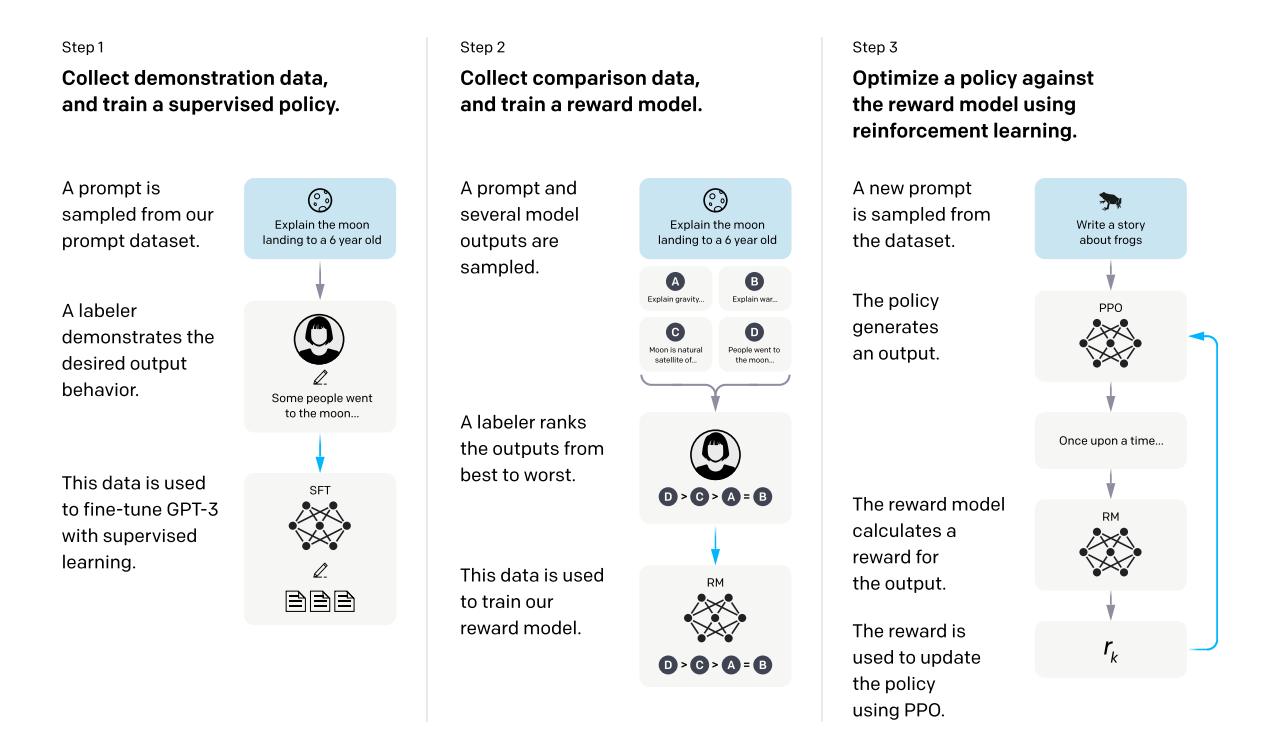
\includegraphics[width=1\linewidth]{InstructGPT.png}
    \caption{The diagram illustrates the three steps of training InstructGPT: (1) supervised fine-tuning (SFT), (2) reward model (RM) training, and (3) reinforcement learning via proximal policy optimization (PPO) on this reward model. }
    \label{fig:enter-label}
\end{figure}

\subsection{Supervised Fine-Tuning (SFT)}
The goal of Supervised Fine-Tuning (SFT) is to train a supervised model on human demonstrations.

The model learns a conditional probability \( \pi_{\text{SFT}}(y^*|x) \), given prompt \(x\) and ideal response \(y*\). The goal is to minimize negative log-likelihood
\[
\mathcal{L}_{\text{SFT}} = -\sum_{t=1}^{T} \log \pi_{\text{SFT}}(y_t | x, y_{<t})
\]

This is defined as the standard cross-entropy loss.

For example, given the prompt \(x\) be "Write three adjectives to describe the ocean", and the human response (i.e., the target \(y*\)) be "vast, deep, tranquil". In the SFT process, it puts the prompt and human response into tokens, and trains the model to learn the conditional probability \( \pi_{\text{SFT}}(y^*|x) \).

   
\subsection{Reward Model (RM) Training}
The goal of Reward Model (RM) training is to train a reward model to mimic human preferences. 

For a given prompt \( x \), pairs of model responses are collected 
\( (y_w, y_l) \), where \( y_w \) is the human-preferred response (winner), while \( y_l \) is the less preferred response (loser).

The reward model \( r_\theta(x, y) \in \mathbb{R} \) assigns scores to outputs. The goal is to train the reward model \(r_\theta\), which minimizes the loss function 
\[
loss(\theta) = -\log\sigma\left(r_\theta(x, y_w) - r_\theta(x, y_l)\right)
\]
Where
\( \sigma(z) = \frac{1}{1+e^{-z}} \) is the sigmoid function. This encourages \( r_\theta(x, y_w) > r_\theta(x, y_l) \).

For example, let the prompt \(x\) be "Write three adjectives to describe the ocean". The model A (\(y_w\)) outputs "vast, deep, tranquil", and the model B (\(y_l\))outputs "high, blue, deep". Human labellers prefer model A to model B, since it is more precise. In the RM training process, the reward function \(r_\theta\) is trained such that \(r_\theta(x, A) > r_\theta(x, B)\).

In the case where each prompt is paired with \(K\) outputs, labellers are asked to rank all \(K\) outputs. In this case, there are \[
\binom{K}{2} = \frac{K(K-1)}{2}
\] pairwise comparisons between all outputs, ans each pair contributes to the loss function. The labellers rank all \( K \) outputs, and the algorithm generates all pairwise comparisons from the ranking (e.g., human labellers rank \(A > B > C\), the pairwise comparisons are \(A > B, A > C\) 
and \(B > C)\). 

The division by \(\binom{K}{2}\) is a normalisation, which ensures the scale of the loss is consistent, regardless of the number of outputs ranked. Without it, prompts with more outputs would disproportionately influence the training. 

The loss function with \(K\) outputs is thus
\[
\text{loss}(\theta) = - \frac{1}{\binom{K}{2}} \mathbb{E}_{(x, y_w, y_l) \sim D} \left[\log \left(\sigma (r_{\theta}(x, y_w) - r_{\theta}(x, y_l)\right)\right]
\]

\subsection{Reinforcement Learning with Proximal Policy Optimisation (PPO)}
Proximal Policy Optimisation (PPO) (\cite{schulman2017ppo}) is an algorithm of Reinforcement Learning (RL). It is a policy gradient method where the agent learns a policy by directly optimising its parameters.
The goal of Proximal Policy Optimisation (PPO) is to train the model to maximise the reward given by the RM (i.e., generate outputs humans prefer, with the reward function).

The objective function is defined as 
\[
\mathbb{E}_{(x,y) \sim \pi_{\text{RL}}} \left[ r_\theta(x, y) - \beta \cdot \log \left( \frac{\pi_{\text{RL}}(y|x)}{\pi_{\text{SFT}}(y|x)} \right) \right] + \gamma \cdot \mathbb{E}_{x \sim D_{\text{pretrain}}} \left[ \log \pi_{\text{RL}}(x) \right]
\]
where
\begin{itemize}
    \item The term \(r_\theta(x, y)\) is the score given by the reward model \(r_\theta\) for the prompt \(x\) and output \(y\). The higher the value, the better the output.
    \item The term \(- \beta \cdot \log \left( \frac{\pi_{\text{RL}}(y|x)}{\pi_{\text{SFT}}(y|x)} \right) \) is the Kullback–Leibler (KL) penalty. It penalises the RL model if it drifts too far from the supervised model \(\pi_{\text{SFT}}\). 
    \item The term \(\gamma \cdot \mathbb{E}_{x \sim D_{\text{pretrain}}}[ \log \pi_{\text{RL}}(x)\) encourages the RL model to retain language modeling capability on pretraining data (Wikipedia, books, etc.), preventing the model from forgetting general knowledge furing training.

\end{itemize}
The aim of PPO is to maximize the expected reward (i.e., objective function).

For example, the prompt is "Tell me something interesting about cats", and the model generates output \(x\) "Cats can rotate their ears 180 degrees". Assume the reward function \(r_\theta (x)\) = 8.2, since it is factual, relevant and phrased clearly;  \(\pi_{\text{RL}}(y|x) = 0.0012\) (i.e., the probability of the RL model gives to this output is 0.0012); \(\pi_{\text{SFT}}(y|x) = 0.0040\) (i.e., the probability assigned by the supervised model to this same response is 0.0040). Thus, the KL penalty is calculated by \[
\log \left( \frac{0.0012}{0.0040} \right) = \log(0.3) \approx -1.204
\]
\[
-\beta \cdot (-1.204) = +1.204\beta
\]
Suppose the sentence is sampled from the pretraining data (e.g., website) and \(\log \pi_{\text{RL}}(x) = -0.15\). Thus, the total reward for this training step is given by \(8.2 +1.204\beta + (-0.15)\gamma\). The PPO optimiser then adjusts model weights to increase the likelihood of output if it is highly rated by the reward model, close to the supervised model, and consistent with general language modelling. 

\section{Relevant work}
The paper surveys the prior work that has motivated InstructGPT, main about improving LLMs through instruction fine-tuning, learning from human preferences, controlling language model behaviour and limitations of supervised fine-tuning. These insights enables the improvement of LLMs training.

\subsection{Improving Language Model Behavior through Instruction Fine-Tuning}
Instead of just scaling up LMs, researchers explored fine-tuning them to follow instructions. Multitask prompted datasets (e.g., SuperGLUE, BigBench) can be used to fine-tune a T5 model. This demonstrated that instruction-tuned models could generalize to unseen tasks with zero-shot prompts. (\cite{wei2021flan}) Besides, relevant papers suggest compiling a large dataset of instructions for NLP tasks and using meta-learning to improve generalization performance. (\cite{sanh2021t0}) This highlighted the value of diverse instruction styles.

\subsection{Learning from human Feedback}
Instead of using ground-truth labels, models can learn from pairwise human comparisons. Existing papers introduced RLHF which trains a reward model on human preferences and optimize a policy using RL (PPO), and InstructGPT directly adopts this method for language modeling. (\cite{christiano2017preferences})

\subsection{Limitationsof supervised fine-tuning}
Supervised learning alone cannot solve instruction alignment, since there exists biases in supervised datasets. (\cite{stiennon2020learning}) RLHF allows training models to optimize what humans actually prefer, not just copy examples. 


\section{Future research directions}
Some possible future research directions in LLM post-training with RL includes diversifying human inputs to reduce RLHF model's biases, improving reward models, combining RLHF with other post-training methods, and improving RL techniques. 

\subsection{Scaling human feedback and aligning with diverse human preferences}
Collecting high-quality human preferences is expensive and doesn’t scale easily. smaller or distilled models (e.g., reward model ensembles or self-critiques) can be used to simulate human preferences. 

Furthermore, current RLHF models reflect the preferences of a small, often homogeneous group of labellers. Fine-tune or condition models on a particular user’s preferences using implicit or explicit signals can be implemented. 

\subsection{Improving reward models \(r_\theta\)}
Reward models can still be noisy. Robust RM Training can be implemented, by using adversarial training or uncertainty modeling to make RMs more stable.

\subsection{Multi-Agent Reinforcement Learning (RL) for Large Language Models (LLMs) Post-Training}
Human's communication is multi-agent, which includes multiple agents with goals, beliefs, and strategies interacting. However, current LLMs optimize in a single-agent setup, ignoring the fact that real-world language use involves coordination, negotiation, and competition. Thus, multi-agent dialogue simulations (e.g., debate, Socratic dialogue, collaborative planning) can be used to refine reasoning, consistency, and social alignment. (\cite{lowe2017marl})



\subsection{Free Energy Principle (FEP) and Large Language Models (LLMs) alignment}
The Free Energy Principle is a neuroscience-inspired theory (\cite{friston2010fep}). It posits that agents act to minimize surprise (or variational free energy) about their sensory inputs — which is a way of modeling the world and predicting outcomes. 

LLMs can be viewed as generative models. Post-training alignment might be improved if models act to reduce uncertainty about user intent, moral context, or task goals. Thus, one possible direction will be actively querying their outputs to reduce ambiguity about what the user wants, instead of passively generating responses.



\bibliography{colm2025_conference}
\bibliographystyle{colm2025_conference}


\end{document}
